\newpage
\section{Parallel Execution}
Python distinguishes between two types of parallelism: multithreading and multiprocessing. Threads provide only an illusion of true parallelism: for a single Python process (i.e., when you run \ls{python your_file.py}) only one thread runs at the same time, but execution switches between multiple threads to create an illusion of parallelism. Even if your script runs on a multi-core (or multi-CPU) machine, only one core will be used\footnote{Since Python version 3.13, the \emph{global interpreter lock} (GIL) which causes  threads to run without true parallelism can be optionally disabled, although the GIL will remain the default behaviour for the forseeable future. See \href{https://docs.python.org/3.13/whatsnew/3.13.html\#whatsnew313-free-threaded-cpython}{here} for more details}. Multiprocessing, on the other hand, can run multiple python processes truly in parallel, simultaneously on more CPU cores if available.

While threads might seem pointless, they are often easier to use and especially for applications which wait on either hardware I/O, network or user interaction they are often the better choice. Multiprocess applications can be faster for sufficiently big problems, however, for short-running programs they are often \emph{slower} because handling of the multiple process introduces \emph{overhead} which can be comparable to the solution of the problem itself.

\subsection{Multithreading}

Threads are represented by \ls{Thread} objects from the \ls{threading} module. Threads execute a given \emph{target} function when they are \emph{started} and after they are finished they have to be \emph{joined} back to the parent thread. Example usage:
\lstinputlisting{../example_code/threads_baisc.py}

However, often an object-oriented approach is more convenient than target functions. We can define our own thread objects by simply inheriting from the \ls{Thread} and defining the \ls{run()} method. A functionally equivalent example to the above:
\lstinputlisting{../example_code/threads_oop.py}

Threads need to be able to communicate with each other and share resources predictably. Consider the VISA \ls{query()} function, which is simply \ls{write()} immediately followed by a \ls{read()}. If there are two threads, communicating with the same pico device, one exectures \ls{query(':READ:P?')} and the the other \ls{query(':READ:T?')} there is a chance that the actual order of executed reads and writes will be
\begin{tabular}{cc}
\begin{lstlisting}[linewidth=0.49\linewidth]
    #thread 1
    write(':READ:P?')
    # thread 2 running
    # thread 2 running
    read()
\end{lstlisting}&
\begin{lstlisting}[linewidth=0.49\linewidth]
    # thread 2
    # thread 1 running
    write(':READ:T?') 
    read()
    # thread 1 running
\end{lstlisting}
\end{tabular}\\
and the thread that asked for pressure will get the temperature and vice versa. This class of bugs is called \emph{race conditions} -- i.e., two threads are "racing" each other to compete for the resource, who wins is random. To avoid this, we need to tell Python that we should not be interrupted for a while until we are done with writing and reading. This is achieved using \emph{locks} (or mutexes, from MUTual EXclusion) which are available in the \ls{threading} module as a \ls{Lock} class as\\
\begin{tabular}{cc}
\begin{lstlisting}
    from threading import Lock
    lock = Lock()
\end{lstlisting}& \\
\begin{lstlisting}[linewidth=0.4\linewidth]
    # thread 1
    lock.acquire()
    # thread 2 running
    write(':READ:P?')
    read()
    lock.release()
    # thread 2 running
    # thread 2 running
    # thread 2 running
\end{lstlisting}&
\begin{lstlisting}[linewidth=0.6\linewidth]
    # thread 2
    # thread 1 running
    lock.acquire() # blocks, until lock is released
    # thread 1 running
    # thread 1 running
    # thread 1 running, lock.acquire() returns
    write(':READ:T?') 
    read()
    lock.release()
\end{lstlisting}
\end{tabular}

Note that we are passing the object created by the \ls{Lock} class rather than the class itself. This is the case for all synchronisation and communication mechanisms -- \ls{Lock}s, \ls{Event}s and \ls{Queue}s and others. Locks support the context management protocol, so typically we use them in the \ls{with} statement rather than calling the \ls{acquire()} and \ls{release()} directly. A more complete example,
\lstinputlisting{../example_code/threads_locks.py}

Note that if we were to use two locks to lock two separate resources we could get into a situation where two locks wait on each other forever such as this\\
\begin{tabular}{cc}
\begin{lstlisting}[linewidth=0.5\linewidth]
    # thread 1
    # tries to acquire lock1 and lock2
    # in this order
    lock1.acquire()
    # thread 2 running
    # thread 2 running
    lock2.acquire() # blocks forever
\end{lstlisting}&
\begin{lstlisting}[linewidth=0.5\linewidth]
    # thread 2
    # tries to acquire lock2 and lock1
    # in this order
    # thread 1 running
    lock2.acquire() 
    lock1.acquire() # blocks forever
    # thread 1 running
\end{lstlisting}
\end{tabular}\\
which is called a \emph{deadlock}. Be extra careful when you use more than one lock.

The simplest method of communicating between threads are global variables. However, this can quickly become messy and confusing therefore it is typically better to use primitives intended for inter-thread communication. The simplest is \ls{threading.Event} which is a boolean flag which can be set by one thread and reacted on by another, e.g.,
\lstinputlisting{../example_code/threads_events.py}

To send data between threads \ls{Queue}s from the module \ls{queue} are useful. We can put a value inside the queue in one thread using the \ls{put()} method and take it out elsewhere using the \ls{get()} method which blocks if the queue is empty. We can also check whether a queue is empty using the \ls{empty()} method. A minimal example
\lstinputlisting{../example_code/threads_queues_minimal.py}

A more complete example that reads data from the pico in one thread and plots it another
\lstinputlisting{../example_code/threads_queues.py}

\begin{exercise}
    Write a program that will flash all 5 LEDs with intervals of 0.1, 0.2, 0.5, 1, and 2 s.
\end{exercise}

\begin{exercise}
    Write a program that will show an updating plot of pressure. While the program runs, it should be able to accept text commands, and it should support: clear, which clears the current plot and quit, which quits the program cleanly.
\end{exercise}

\subsection{Multiprocessing}
Multiprocessing can use multiple CPU cores, however, there are restrictions on what kind of variables can be shared between processes. We can create new processes using the \ls{Process} class from the \ls{multiprocessing} module in a very similar manner to threads. The \ls{multiprocessing} module also provides synchronisation and communication facilities similar to \ls{threading}, i.e., \ls{Event}, \ls{Queue} etc. However, you must use the classes in the multiprocessing module to communicate between processes. A minimal example, where the main process creates a set of processes and sends messages to them all through a shared \ls{Queue}
\lstinputlisting{../example_code/multiprocessing_process.py}

The above code is an example of a \emph{process pool}, which is often the simplest way to speed up problems which involve multiple independent calculations. Multiprocessing already provides a general process pool precisely for this task
\lstinputlisting{../example_code/process_pools_minimal.py}
which applies the function \ls{function(x)} to every element of the sequence (e.g., list, array, ...) in 6 parallel processes collecting the results.

A more complete example that calculates the Fibonacci sequence,
\lstinputlisting{../example_code/process_pools.py}
notice that for large number of processes the calculation actually takes \emph{longer}.

\subsection{Inter-process Communication}
So far we created new processes from a python script which we ran. However, any two python processes, i.e., separate runs of any python programs, can communicate with each other. There are several ways achieve this, such as directly sharing memory (using \ls{multiprocessing.shared_memory} module, see \href{https://docs.python.org/3/library/multiprocessing.shared_memory.html}{the documentation} for example use with numpy arrays) or \emph{sockets}. Socket mechanism is in some way provided by all operating systems as a general way of communication between processes, locally or over network, see Fig.~\ref{fig:listener-client}. Generally, we establish a connection with an address (can be \emph{localhost} if not communicating over network) and a port number. One process acts as the \emph{listener} (i.e., server) which \emph{accepts} connections from \emph{clients} and the two can then send messages to and receive messages from each other.

\begin{figure}
    \label{fig:listener-client}
    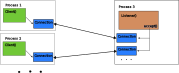
\includegraphics[width=\textwidth]{listener_client.pdf}
    \caption{Relationships between Listeners, Clients and Connections}
\end{figure}

The example below shows a simple echo server -- a server that simply sends back to the client what it receives. It will only accept connections from the local computer on the port 6000. First, the listener object is created using the \ls{with} statement, which is then used to start a separate thread which accepts the connections and responds to clients. The main thread will simply wait for the signal to quit. If we are supposed to quite, close the listener (we also need to unblock the \ls{accept()} which would wait forever) and quit. Note that the passwords are optional, if you do not specify the \ls{authkey} for the \ls{Listener}, you also do not have to specify it for \ls{Client}.

The client is in comparison much simpler. Simply connect to the listener with known address, port and password, and you can start sending and receiving data. Note that \ls{send()} and \ls{recv()} pickle and unpickle (recall pickling from \ls{.npy} files), so almost all Python-objects can be sent.

To test the example below, run \verb|python server.py| in one console and \verb|python client.py| in another.

\ls{server.py}:
\lstinputlisting{../example_code/ipc_server.py}

\ls{client.py}
\lstinputlisting{../example_code/ipc_client.py}

To allow connections from the network, simply specify the Listener address as \ls{''} (empty string) and the connect with the client to the IP address of the computer running the listener process. Note that pickling and unpickling in \ls{send()} and \ls{recv()} can lead to potential security issues, so it is best to use a password if accepting connections over the network.

\begin{exercise}
A server is running on computer with IP address \verb|<IP>|, on port \verb|<PORT>| with password \verb|<PASSWORD>|. This server is controlling a Pico by directly sending whatever string it receives to the pico and sending the response from the pico back. Connect to this server with a client, send the command \verb|*IDN?| to query the instrument's identification and blink an LED if the response is correct.
\end{exercise}

\verb|instrument_server.py|:
The code accepts the connections in a separate thread. For each connection it accepts, it starts a new client handler thread. All client handler threahds share the same pico, so we have to lock it appropriately before attempting communication, because another client can interrupt us at any moment. The server quits when it receives KeyboardInterrupt (Ctrl-C) 
\lstinputlisting{../example_code/instrument_server.py} %

\subsubsection{Real use case in a lab}
In Fig.~\ref{fig:networking-usecase} is a photo of a single computer which controls three experiments connected to two different experimental setups. Each experiment belongs to a different student, who might need to run and modify their measurement Python scripts at the same time, so simple remote desktop sharing is not available.

We ended up using an instrument server similar to the simplified example above, which allowed the students to run the measurement scripts on any computer on the same network, even on their own laptops.

\begin{figure}
    \label{fig:networking-usecase}
    TODO
    \caption{Single computer controlling multiple experiments.}
\end{figure}